\documentclass{article}
\usepackage[frenchb]{babel}
\usepackage[utf8]{inputenc}
\usepackage[T1]{fontenc}
\usepackage{amsmath}
\usepackage{minted}
\usepackage{graphics}
\usepackage{hyperref}

\title{Recherche de chemin --- Algorithme de Dijkstra avec tas de Fibonacci et applications}
\author{Corentin Cadiou \and Lucas Verney}

\begin{document}
\maketitle
Le but de ce projet était de réaliser une implémentation de
l'algorithme de Dijkstra de recherche de chemin en utilisant des tas de
Fibonacci.

Cette implémentation a été réalisée dans le langage C et est détaillée
dans les Sections~\ref{sec:algor-de-dijkstra}
et~\ref{sec:tas-de-fibonacci}. Un ``\emph{wrapper}'' python3 a été
créé pour pouvoir interagir facilement avec l'algorithme, comme
détaille dans la Section~\ref{sec:expos-des-fonct}. Enfin, un script
Python qui lit une carte OpenStreetMap, le convertit en un format
d'entrée correct pour notre implémentation et effectue des recherches
dedans a été écrit.

\section{Algorithme de Dijkstra}\label{sec:algor-de-dijkstra}
L'algorithme étudié est l'algorithme de Dijkstra. Cet algorithme a
une complexité algorithmique de $O(|E| + |V|\log|C|)$ dans le cas
d'une implémentation avec une queue de priorité, comme par exemple
avec un tas de Fibonacci (ou une queue de Brodal).

Le principe de l'algorithme est de parcourir progressivement tout le
graphe. On ajoute initialement tous les nœuds associés à une distance
infinie à une file de priorité. La source est attribuée à une distance
nulle. On initialise de plus une liste contenant les nœuds déjà visités.

On itère ensuite sur la file de priorité jusqu'à ce qu'elle soit vide.
À chaque itération, le nœud $u$ de la file le plus proche de la source
est extrait de la file et marqué comme visité.
Pour tous ses voisins $v$ non déjà visités, on
calcule la distance du chemin allant de la source $v$ en passant par
$u$. S'il est plus faible que la distance de $v$ à la source sans passer
par $v$, on met à jour cette distance et on note que le prédécesseur
de $v$ est $u$.

Une preuve (succincte et partielle) que l'algorithme est correcte est
donnée ci-dessous. On peut le prouver en supposant que
l'itération marque les nœuds visités avec la distance minimale et que
tous les nœuds non visités sont plus loin que la plus faible des
distances dans la file de priorité.
À l'itération suivante, un nœud voisin du nœud dans la file le plus
proche de la source est sélectionné, sa distance est mise à jour. S'il
devient alors l'élément le plus proche de la source, il ne peut être
atteint en moins de distance depuis les nœuds visités dans la file
puisqu'il est plus proche que tous les autres. De même, il n'est pas
atteignable par un nœud non encore visité, par hypothèse. S'il n'est
pas le plus proche, soit il existe un chemin plus court l'atteignant
et il sera alors trouvé, soit le chemin proposé initialement était le
bon et on le saura quand tous les nœuds dans la file seront à une
distance supérieure que celle calculée. On a donc conservé l'hypothèse
par itération.
Comme celle-ci est vraie pour la première itération (la distance la
plus courte de la source à ses voisin est la distance entre ceux-ci),
elle est vraie pour toutes les itérations. On ax donc trouvé la plus
courte distance entre la source et chacun des nœuds du graphe.

On peut implémenter l'algorithme avec une queue supportant les trois
opérations suivantes :
\begin{enumerate}
  \item ajout d'une clé (la distance du nœud du bout à la source), avec
    décoration (les deux nœuds formant l'arête)
    \mint{python}|insert(from, to, distance)|
  \item récupération du minimum et suppression de la file
    \mint{python}|extract_min()|
\end{enumerate}
\begin{minted}[linenos,frame=lines]{python}
def Dijkstra(Graph, source):            # Source is the startpoint of the algorithm
   dist[source] = 0                     # Initialisation
   for vertex v in Graph:
       if v != source:
           dist[v]     = Infinity       # Unknown distance from source to v
           previous[v] = None           # Predecessor of v

   source.mark = scanned

   # Initialise the queue with the neighbours of the source
   for u in source.neighbours:
       d = dist[source] + length(source, u)
       Q.insert(u, v, d)

   while Q is not empty:                # The main loop
       u, v, d = Q.extract_min()        # Remove and return best vertex
       if v.mark is not scanned:
           dist[v] = d
           prev[v] = u
           v.mark = scanned

           for w in v.neighbours:
               d = dist[v] + length(v, w)
               Q.insert(v, w, d)
   return previous
\end{minted}
\section{Tas de Fibonacci}\label{sec:tas-de-fibonacci}
  Les tas de Fibonacci supportent les mêmes opérations que les tas binomiaux, vus en cours, avec l'avantage que toutes les opérations qui ne nécessitent pas la suppression d'un élément s'exécutent en temps $O(1)$.

  Un tas de Fibonacci est un ensemble d'arbres ordonnées, non triés. Chaque nœud $x$ contient un pointeur \texttt{x.parent} vers son père, \texttt{x.child} vers n'importe lequel de ses fils. Il possède en outre deux pointeurs \texttt{x.left} et \texttt{x.right} vers ses frères gauche et droite respectivement. Tous les enfants d'un nœud forment ainsi une liste circulaire doublement chaînée. Dans le cas particulier d'un fils unique, on a donc \texttt{x.left = x.right = x}.

  Grâce à cette structure de listes circulaires doublement chaînées, un nœud peut être supprimé en temps $O(1)$.

  Enfin, chaque nœud a un dernier champ, en plus des décorations éventuelles liées à notre utilisation, \texttt{x.degre} qui stocke le nombre d'enfants qu'il a.

  Le tas en lui-même comporte deux éléments particuliers : un pointeur sur l'élément minimal, \texttt{fh.min}, et un pointeur sur n'importe laquelle des racines, \texttt{fh.root}. Le pointeur sur l'élément minimal nous permet de trouver le minimum dans le tas en temps $O(1)$. Les racines, comme tous les autres nœuds, sont reliées entre elles dans une liste doublement chaînée.

  Les opérations d'insertion et d'extraction du minimum sont implémentées comme décrites en pseudo-code dans Charles E Leiserson, Ronald L Rivest, Clifford Stein, and Thomas H Cormen. \emph{Introduction to algorithms}. The MIT press, 2001.

  Une opération d'insertion se fait en temps $O(1)$, Une opération d'extraction du minimum se fait en temps $O(D(n))$ où $D(n)$ est un majorant du degré maximal d'un nœud. D'après la référence précédente, celui-ci est borné par $\log_\varphi \left(n\right)$ où $n$ est le nombre total de nœuds dans le tas de Fibonacci, donc l'extraction de l'élément minimal est en $O(\log n)$.

\section{Exposition des fonctionnalités en
  Python}\label{sec:expos-des-fonct}
Pour rendre l'interaction avec l'algorithme plus aisée ainsi que pour
profiter des fonctionnalités plus haut niveau de Python, non
pertinentes d'un point de vue algorithmique (comme la lecture d'un
fichier XML), un ``\emph{wrapper}'' python a été écrit en utilisant
\texttt{Cython}. Ce ``\emph{wrapper}'' expose une classe python appelée \verb|Graph|
représentant un graphe et qui donne accès au nombre de nœuds
(\verb|nb_vertices|), propose une méthode pour ajouter des arêtes
(\verb|addEdge|) ainsi que pour afficher le graphe ou les voisins d'un
nœud (\verb|get|). La méthode appelle en réalité des fonctions C et
s'occupe uniquement de l'interfaçage entre les deux langages.

La classe propose aussi une méthode \verb|dijkstra| qui lance
l'algorithme sur le graphe construit. On a donc exposé entièrement
tous les outils nécessaires à l'exploitation de l'algorithme. On
trouvera le code dans l'Annexe~\ref{sec:code-du-wrapper}.
\section{Application: recherche de chemin vers les transports publics
  les plus proches}\label{sec:appl-rech-de}
  Une fois le ``\emph{wrapper}'' écrit, il a été possible d'utiliser les
fonctionnalités haut niveau de Python comme la lecture du format XML
(pour les cartes OpenStreetMap) et du JSON (pour les requêtes de l'API
OpenStreetMap pour trouver les adresses).

Pour cela, le script Python commence par lire le fichier OSM. Il
récupère toutes les balises \verb|node| au format :
\begin{minted}{xml}
<node id="703217417" lat="48.8445203" lon="2.3439455" ... />
\end{minted}
et les renumérote entre $0$ et $n_\mathrm{nodes}-1$. Ces \verb|node|
seront considérés comme les nœuds du graphe. Elles correspondent à des
intersections de rues ou des points particuliers (arrêts de bus,
monuments, limites d'un bâtiment, ).

La deuxième étape consiste à ajouter au graphe les arêtes,
c'est-à-dire les routes. Celles-ci sont représentées comme suit :
\begin{minted}{xml}
<way id="4217181" visible="true" …>
 <nd ref="25033471"/> <!-- Intersection rue d'Ulm, rue Érasme -->
 <nd ref="25033484"/>
 <nd ref="25033485"/>
 <tag k="highway" v="residential"/>
 <tag k="name" v="Rue Érasme"/>
</way>
\end{minted}
Le chemin est formé d'une ligne brisée composée par la succession des nodes.
Les routes n'ayant pas de \verb|tag| avec la valeur \verb|k="highway"|
ne sont pas considérés (ce sont des bâtiments, des monuments, …). Nous
avons ajouté au graphe chacun des couples successifs de \verb|nodes|, avec
comme distance\footnote{Se référer à l'article Wikipédia correspondant pour plus d'informations sur cette distance : \url{https://en.wikipedia.org/wiki/Haversine_formula}} :
\begin{align*}
  D & = 2 R_\mathrm{earth}\ \mathrm{atan} \left( \frac{\sqrt{a}}{\sqrt{1-a}} \right) \\
  a & = \left( \frac{\sin(\Delta_\mathrm{lat})}{2} \right)^2 +
      \cos(\mathrm{lat_1})\cos(\mathrm{lat_2}) \left( \frac{\sin(\Delta_\mathrm{lon})}{2} \right)^2
\end{align*}

\section{Vérification de la complexité de l'algorithme}
Nous avons vérifié que l'implémentation de l'algorithme de Dijkstra
utilisant une file de priorité naïve s'effectue en temps $O(|U| + |V|^2)$ tandis
que l'implémentation avec les tas de Fibonacci s'effectue en temps
$O(|E| + |V|\log |V|)$. Pour cela, nous avons généré des graphes
d'Erdös-Rényii de taille entre 10 et 10000 sommets avec $p$ pris uniformément (aléatoirement, pour chaque génération) entre 0 et 1. Les courbes du temps de travail de l'algorithme ont ensuite été
tracées. Les résultats montrent qu'effectivement, la
non-implémentation des tas de Fibonacci mène à une complexité en
$O(|U| + |V|^2)$ comme montré sur la Figure~\ref{fig:reg_queue}. Pour
les tas de Fibonacci, on obtient bien un temps amorti en $O(|E| +
|V|\log |V|)$ comme on peut l'observer sur la Figure~\ref{fig:reg_fib}.

\begin{figure}
  \begin{center}
    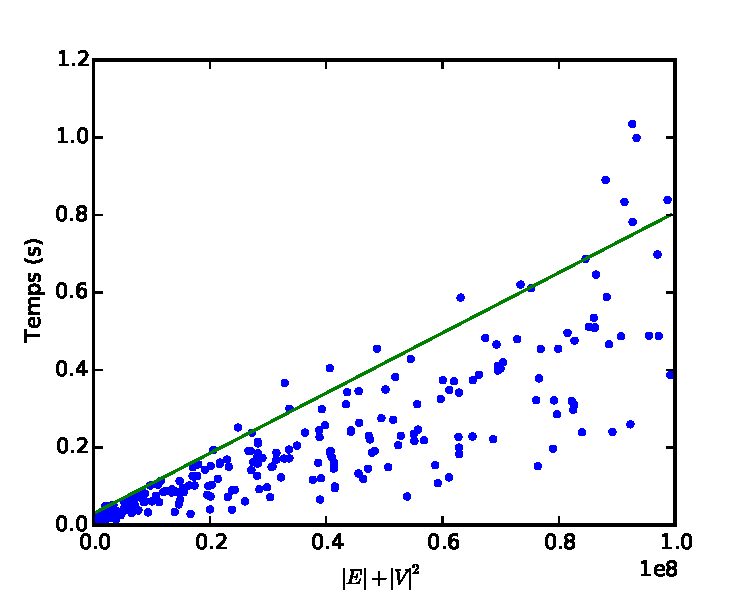
\includegraphics{reg_queue.pdf}
  \end{center}
  \caption{\label{fig:reg_queue}Courbe du temps en fonction de
    $|E| + |V|^2$ en utilisant un tas simple.
    On constate que tous les points se situent en
    dessous de la droite, ce qui correspond bien à la définition d'un
    temps en $O(|E| + |V|^2)$.}
\end{figure}
\begin{figure}
  \begin{center}
    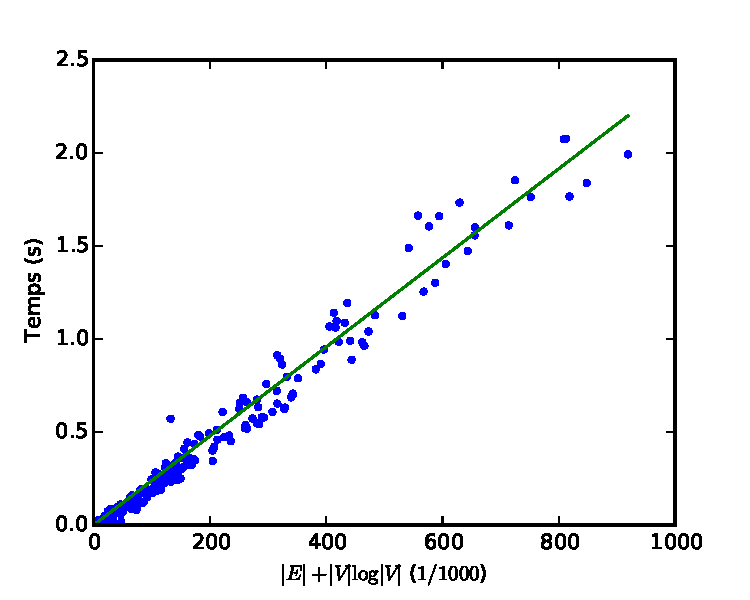
\includegraphics{reg.pdf}
  \end{center}
  \caption{\label{fig:reg_fib}Courbe du temps en fonction de
    $|E| + |V|\log |V|$ en utilisant les tas de Fibonacci.
    On constate que tous les points se situent en
    dessous de la droite, ce qui correspond bien à la définition d'un
    temps en $O(|E| + |V|\log |V|)$.}
\end{figure}

Enfin des tests de perfomance ont été effectués sur des cartes
OSM. Les résultats sont largement en la faveur des tas de Fibonacci,
comme on peut le constater dans le tableau~\ref{tab:comp_osm}.
\begin{table}[htbp]
      \centering
      \begin{tabular}{clrrr}
        Carte & Nœuds & Arêtes & Temps -- Fibonacci (ms) & Temps -- tas
                                                     simple (ms)\\
        \hline
        1 & 3,724 & 722 & 0.38 & 38 \\
        2 & 15,253 & 1,908 & 1.2 & 632 \\
        3 & 50,313 & 8,588 & 7.2   & 7,116 \\
        4 & 171,153 & 29,578 & 29.8 & 84,524
      \end{tabular}
      \caption{\label{tab:comp_osm}Comparaison des temps d'exécution de l'algorithme de
        Dijkstra selon l'implémentation du tas utilisée.} 
    \end{table}
\appendix
\section{Code du \emph{wrapper}}\label{sec:code-du-wrapper}
Le \emph{wrapper} utilise deux classes, l'une en \texttt{Cython} (lignes 7 à 72) qui
interagit directement avec le code C et l'autre en Python pur (lignes
75 à 109), qui interagit avec la classe \texttt{Cython} (celle-ci ne permettant
pas d'utiliser toutes les fonctionnalités de Python). ``\texttt{from pyjkstra cimport …}''
est une routine \texttt{Cython} qui importe le fichier ``pyjkstra.pxd''
contenant les \emph{headers} dans lesquels trouver les fonctions C appelées.
\begin{minted}[linenos,frame=lines]{cython}
from libc.stdlib cimport malloc, free
from cpython cimport array
from pyjkstra cimport dijkstra as c_dijkstra
from pyjkstra cimport graph_t, createGraph, freeGraph
from pyjkstra cimport printGraph, printNode, addEdge, INT_MAX

cdef class c_Graph:
    '''Cython class that exposes a graph'''
    cdef graph_t * thisptr

    def __cinit__(self, int n):
        ''' Initialises a C pointer to the graph structure.'''
        self.thisptr = createGraph(n)
        if self.thisptr is NULL:
            raise MemoryError

    def __dealloc__(self):
        ''' Free the malloced memory. '''
        if self.thisptr is not NULL:
            freeGraph(self.thisptr)

    def __str__(self):
        ''' Print a representation of self.'''
        # Bad hack, it prints but returns an empty string …
        printGraph(self.thisptr)
        return ""

    @property
    def nb_vertices(self):
        return self.thisptr.nb_vertices

    def get(self, int n):
        printNode(self.thisptr, n)

    def addEdge(self, int src, int dest, double weight):
        addEdge(self.thisptr, src, dest, weight)

    def dijkstra (self, int s):
        ''' Converts the Python objects to and from C variables and
        call the algorithm. '''

        cdef int l = self.thisptr.nb_vertices

        # Malloc arrays for return values of the dijkstra algorithm
        cdef int* prev_arg = <int*>malloc(sizeof(int)*l)
        cdef double* dist_arg = <double*>malloc(sizeof(double)*l)

        # Call the algorithm
        c_dijkstra(self.thisptr, s, prev_arg, dist_arg)

        prev_out = []
        dist_out = []
        # Convert back from C-types to python object
        for i in range(l):
            if (prev_arg[i] == INT_MAX):
                val = None
            else:
                val = prev_arg[i]

            prev_out.append(val)


            if (dist_arg[i] == INT_MAX):
                val = None
            else:
                val = dist_arg[i]

            dist_out.append(val)

        # Free C arrays
        free(dist_arg)
        free(prev_arg)
        return (prev_out, dist_out)

# This is the pure Python class that implements all "methods" of our graph
class Graph:
    ''' A graph represented as an adjacency list.'''
    c_graph = None
    def __init__(self, int n):
        ''' n is the number of vertices.'''
        self.c_graph = c_Graph(n)

    def __del__(self):
        del self.c_graph

    def __str__(self):
        return self.c_graph.__str__()

    @property
    def nb_vertices(self):
        return self.c_graph.nb_vertices

    def addEdge(self, int src, int dest, double weight):
        ''' Adds an edge to the graph from `src` to `dest` with weight `weight`.'''
        self.c_graph.addEdge(src, dest, weight)

    def get(self, int n):
        return self.c_graph.get(n)

    def dijkstra (self, int s):
        ''' Implement the dijkstra path-finding algorithm.
        Parameters:
        G    dijkstra.Graph    a python representation of a graph
        s    int               the starting point of the algorithm

        Returns:
        (prev, dist) with prev the antecedent in the path and dist the distance of
        each node from the start
        '''
        return self.c_graph.dijkstra(s)
\end{minted}

\section*{}
\end{document}
